\documentclass[11pt]{article}
\usepackage[margin=1in]{geometry}
\usepackage{booktabs}
\usepackage{graphicx}
\usepackage{hyperref}

\title{CAI6734 Weekly Report 9: A Contrastive Hypothesis Agent That Learns Alongside the Decision Agent}
\author{Omer Kahveci}
\date{November 24, 2026}

\begin{document}
\maketitle

\section{Project Objective}

Week 8 located the bottleneck of our LA-CDM reproduction. The Decision Agent's
(DA's) test choices were already good (H1). A Hypothesis Agent (HA) fine-tuned
on its own was a better diagnoser than the HA inside the shared adapter (H2).
Retraining the DA against that frozen HA kept accuracy and cut cost by about
20\% (H3a).

After the Week 8 report, it was suggested in our meeting to try a \emph{Contrastive Language
Model} (CLM) as the HA: a model that maps the patient's state and the possible
final outputs into one embedding space. This also allowed us to revisit the
original idea of LA-CDM, that both agents learn \emph{together}, with an HA
that is cheap to update during the DA's training. I pre-registered the plan as
H4 before any result existed:

\begin{itemize}
  \item \textbf{H4a:} is a CLM-style HA as good a diagnoser as our best HA?
  \item \textbf{H4b:} what happens when it replaces the HA next to the baseline
        DA, without retraining? (Informative only.)
  \item \textbf{H4c:} when a new DA is trained with the CLM HA, does letting the
        HA keep learning during training (``joint'') beat keeping it frozen?
\end{itemize}

\section{Accomplishments}

\subsection*{My Contributions This Week}

\begin{itemize}
  \item Studied contrastive language models (Contrastive-LM, Kwok et al.,
        2026) and adapted the method to our Llama backbone.
  \item Implemented the CLM HA: embedding of every patient record with a frozen
        Llama, contrastive projection heads, head training with validation-based
        selection, and test scoring in the same format as the H2 HAs.
  \item Integrated the CLM HA into the LA-CDM environment, including online
        updates of the heads after every DA training step, with saving and
        resuming of the heads and their optimizer.
  \item Ran H4a, H4b and H4c (two 700-step DA training runs) and computed paired
        statistics for all three.
  \item Found and fixed a bug in resuming training runs that use two adapters,
        which also corrects a conclusion of Week 8 (Section~\ref{sec:challenges}).
  \item Built figure scripts for H3 and H4.
\end{itemize}

All comparisons use the same 240 test patients, paired tests (exact McNemar for
accuracy, paired bootstrap for intervals) and 95\% confidence intervals.
Checkpoints, epochs and backbones were always chosen on validation.

\textbf{Names used below.} I renamed the Week 8 ``new HA'' to make clear how it
differs from the others.
\begin{itemize}
  \item \textbf{Baseline model:} our LA-CDM reproduction (85.4\% accuracy). Its
        \emph{baseline DA} and \emph{baseline HA} share one LoRA adapter and are
        trained jointly.
  \item \textbf{Separately fine-tuned HA:} the HA fine-tuned on its own in H2
        (seed 0), then frozen. Called the ``new HA'' in Week 8.
  \item \textbf{CLM HA:} the contrastive HA built this week (below).
  \item \textbf{H3a:} a DA retrained against the frozen separately fine-tuned
        HA (Week 8).
\end{itemize}

\subsection*{How the CLM HA Works}

The HA has to choose one of four diseases from a partial patient record. The
CLM HA does this by comparing vectors instead of generating text:

\begin{enumerate}
  \item A frozen Llama-3-8B reads the HA prompt (history and test results so
        far) and returns its hidden state at the last token: one vector of
        4,096 numbers that summarises the record. It also reads each of the four
        texts ``Final diagnosis: \emph{disease}''.
  \item Two small projection heads (about 7M parameters each) map the record
        vector and the four disease vectors into one shared 512-dimensional
        space.
  \item The cosine similarities, multiplied by a learned temperature, give four
        scores; a softmax turns them into the HA's probabilities.
  \item The heads are trained with a contrastive (InfoNCE) loss, which pulls
        each record towards its true disease and pushes it away from the other
        three. Llama itself is never trained.
\end{enumerate}

I tried two frozen backbones: plain Llama, and Llama with the separately
fine-tuned HA's adapter. The heads were trained on the same 7,676 training
records as the separately fine-tuned HA: up to four distinct views of each
training patient (history only, all tests, and two random subsets of tests),
and 720 validation records. The
adapter backbone reached 86.9\% validation accuracy (best epoch 2), against
80.0\% for plain Llama (epoch 21), so it was chosen. Contrastive-LM trains its
heads on a Qwen model with about 90 million examples, so I did not use their
released heads; this tests the method, not their checkpoint.

\subsection*{H4a: The CLM HA Matches the Best HA}

The rule, fixed in advance: on the baseline DA's records, the CLM HA is
\emph{better} if the 95\% interval of its accuracy gain over the separately
fine-tuned HA is above zero, and \emph{not worse} (non-inferior) if the lower
bound is above $-$3 points. If it were worse, H4c would not be run with it.

\begin{table}[ht]
  \centering
  \caption{H4a: accuracy of each HA on identical records (as in Week 8,
  Table~2). Columns give the test results shown to every HA: none; random
  tests, as many as the baseline DA ordered; the tests the baseline DA ordered;
  or every available test. Each HA's answer is its highest-probability disease.
  ECE is with all tests.}
  \label{tab:h4a}
  \small
  \begin{tabular}{lrrrrr}
    \toprule
    HA & No tests & Random & Baseline DA's & All tests & ECE \\
    \midrule
    Untrained model (zero-shot) & 61.3\% & 63.3\% & 82.5\% & 75.4\% & 10.8\% \\
    Baseline HA (shared adapter) & 63.3\% & 64.6\% & 87.9\% & 87.9\% & 5.6\% \\
    Separately fine-tuned HA & 78.3\% & 80.8\% & 88.8\% & 90.0\% & 4.5\% \\
    CLM HA, plain Llama & 70.8\% & 73.3\% & 85.4\% & 85.4\% & 6.8\% \\
    CLM HA, fine-tuned (chosen) & 77.1\% & 80.0\% & 89.2\% & 90.8\% & 4.9\% \\
    \bottomrule
  \end{tabular}
\end{table}

\begin{figure}[htbp]
  \centering
  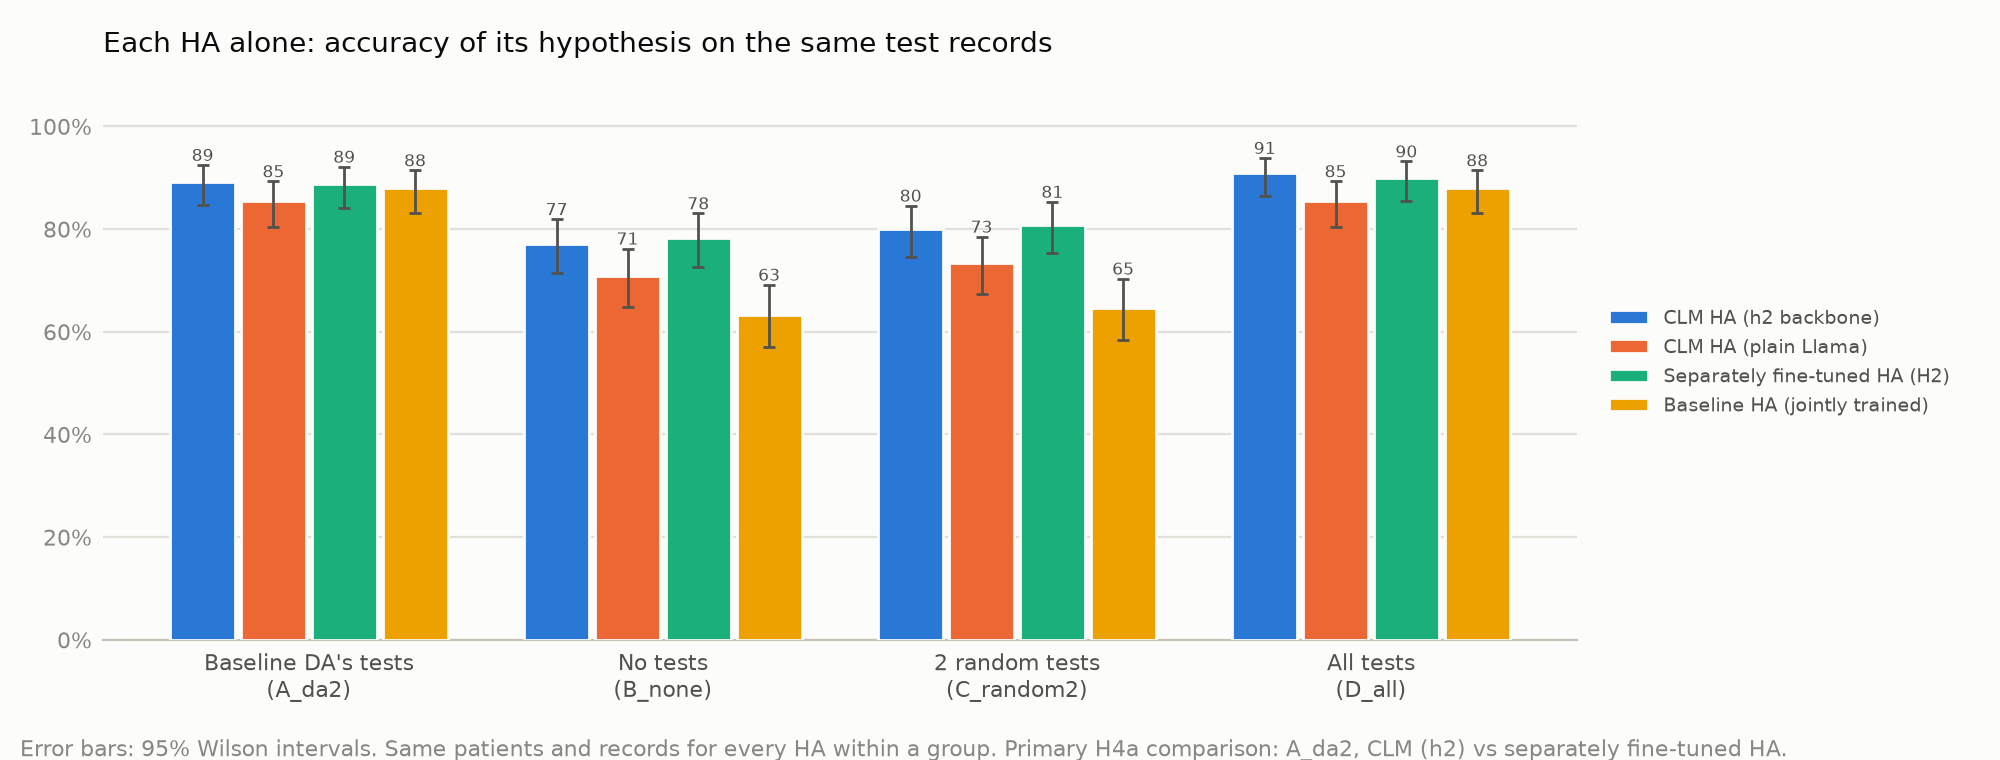
\includegraphics[width=\textwidth]{h4_ha_test.png}
  \caption{H4a: each HA alone on the same test records, with 95\% Wilson
  intervals.}
  \label{fig:h4a}
\end{figure}

\textbf{H4a: not worse.} On the baseline DA's records the CLM HA was ahead by
+0.4 points [$-$1.3, +2.1] ($p = 1.00$; the two HAs disagreed on only 5 of 240
patients). The interval includes zero, so it is not better, but its lower bound
is above $-$3, so it is not worse. On the other record sets it was within 1.2
points of the separately fine-tuned HA as well (Table~\ref{tab:h4a}; these were
secondary and not tested separately). On the
baseline DA's records its calibration was slightly worse (ECE 6.3\% against
4.6\%). The close agreement is expected, and it limits what H4a shows: the chosen
heads read the separately fine-tuned HA's own representation, so most of the
CLM HA's accuracy is inherited from that HA rather than added by the contrastive
heads. The CLM on its own is better judged by the plain-Llama version: with only
the trained heads and no fine-tuning of the language model at all, it reached
85.4\% on the baseline DA's records, below both the baseline HA (87.9\%) and the
separately fine-tuned HA (88.8\%).

\subsection*{H4b: The Baseline DA with the CLM HA}

\begin{table}[ht]
  \centering
  \caption{H4b: the baseline DA (no retraining) with three different HAs.
  ``DA'' is the accuracy of the DA's diagnosis, ``HA'' that of the HA's last
  hypothesis; cost is per case; AUROC measures how well the HA's confidence
  separates its correct from its wrong hypotheses.}
  \label{tab:h4b}
  \small
  \begin{tabular}{lrrrrr}
    \toprule
    HA next to the baseline DA & DA & HA & Cost & ECE & AUROC \\
    \midrule
    Baseline HA (baseline model) & 85.4\% & 87.1\% & \$1,259 & 14.8\% & 0.750 \\
    Separately fine-tuned HA & 85.4\% & 89.2\% & \$1,285 & 5.2\% & 0.936 \\
    CLM HA & 82.9\% & 88.8\% & \$1,235 & 8.1\% & 0.915 \\
    \bottomrule
  \end{tabular}
\end{table}

With the CLM HA the baseline DA's accuracy was 2.5 points lower than with the
separately fine-tuned HA [$-$5.4, +0.4] ($p = 0.15$), a difference that is not
significant. A small drop is plausible because this DA was trained reading the
baseline HA's messages. The CLM HA's confidence was far more informative than the
baseline HA's (AUROC 0.915 against 0.750), but slightly less than the
separately fine-tuned HA's. This comparison was informative only and decided nothing.

\subsection*{H4c: Does a Learning HA Help the DA?}

H4c trains a new DA from the untrained model against the CLM HA, in two arms
that differ only in the heads:

\begin{itemize}
  \item \textbf{Joint:} after every DA step the heads take one small update on
        the records that step produced (labelled with the true disease), mixed
        with 32 random training records so they do not forget.
  \item \textbf{Frozen:} the same heads, never updated.
\end{itemize}

Llama stays frozen in both arms. Each arm trained for 700 steps (one patient and
four rollouts per step, about 36\% of the training patients), the same budget
as H3a. The rule: joint is supported only if the 95\% interval of ``joint minus
frozen'' on the DA's accuracy is entirely above zero. Each arm's step was chosen
on validation (Figure~\ref{fig:h4val}): step 600 for joint (73.6\%) and step 400
for frozen (70.0\%). During training the heads' online loss stayed low (about
0.05 at the end), so the heads did not drift.

\begin{figure}[htbp]
  \centering
  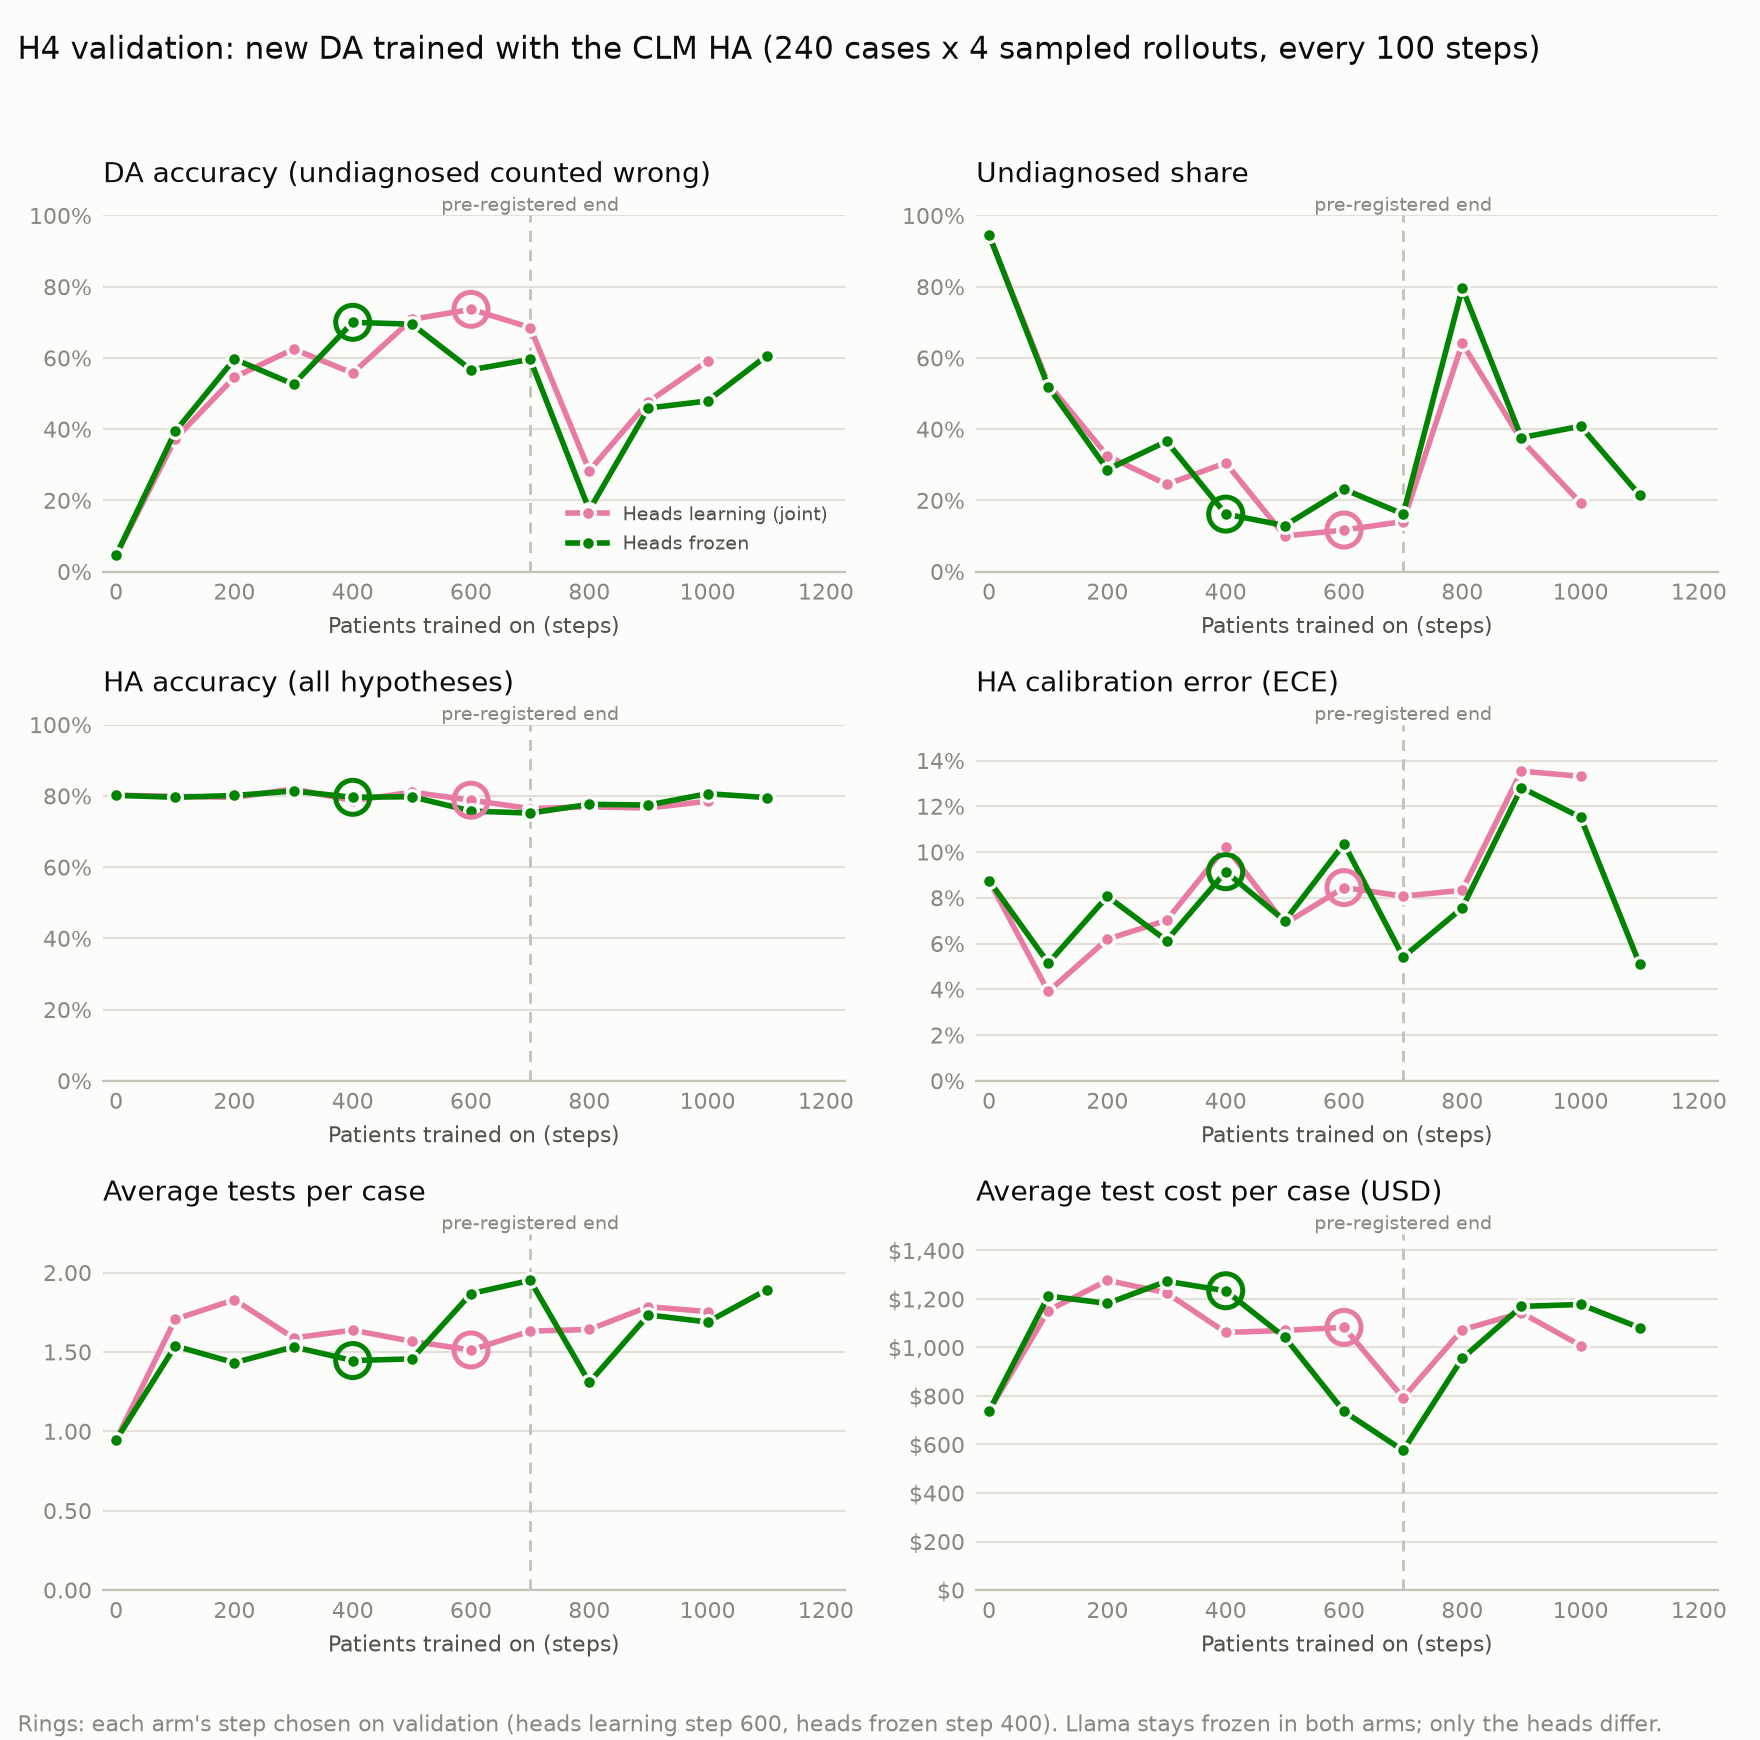
\includegraphics[width=\textwidth]{h4_validation.png}
  \caption{H4c validation curves (240 patients, four sampled rollouts each,
  every 100 steps). Rings mark each arm's chosen step.}
  \label{fig:h4val}
\end{figure}

\begin{table}[ht]
  \centering
  \caption{H4c test results (240 cases), with H3a for reference. ``DA'' is the
  accuracy of the DA's diagnosis, ``HA'' that of the HA's last hypothesis; tests
  and cost are per case. H3a is the retrained DA with the separately fine-tuned
  HA.}
  \label{tab:h4c}
  \small
  \begin{tabular}{lrrrr}
    \toprule
    System (chosen step) & DA & HA & Tests & Cost \\
    \midrule
    New DA + CLM HA, joint (600) & 84.2\% & 87.5\% & 1.39 & \$1,189 \\
    New DA + CLM HA, frozen (400) & 82.1\% & 88.8\% & 1.50 & \$1,434 \\
    H3a (700) & 85.8\% & 88.3\% & 1.27 & \$1,025 \\
    \bottomrule
  \end{tabular}
\end{table}

\textbf{H4c: no detectable gain.} Joint minus frozen was +2.1 points
[$-$2.5, +6.7] ($p = 0.47$), so under the pre-registered rule learning together
did not help detectably. The joint arm was \$245 cheaper per case [$-$\$336,
$-$\$161], but the arms were tested at different steps (600 against 400), so
this difference may come from how far each DA had trained rather than from the
heads. The joint arm was not better than H3a either: $-$1.7 points
[$-$5.4, +2.1] in accuracy and \$164 more per case [+\$95, +\$235]. Its
class-mean accuracy (81.3\%) equals the paper's LA-CDM result at a lower cost
(\$1,189 against \$1,296).

\begin{figure}[htbp]
  \centering
  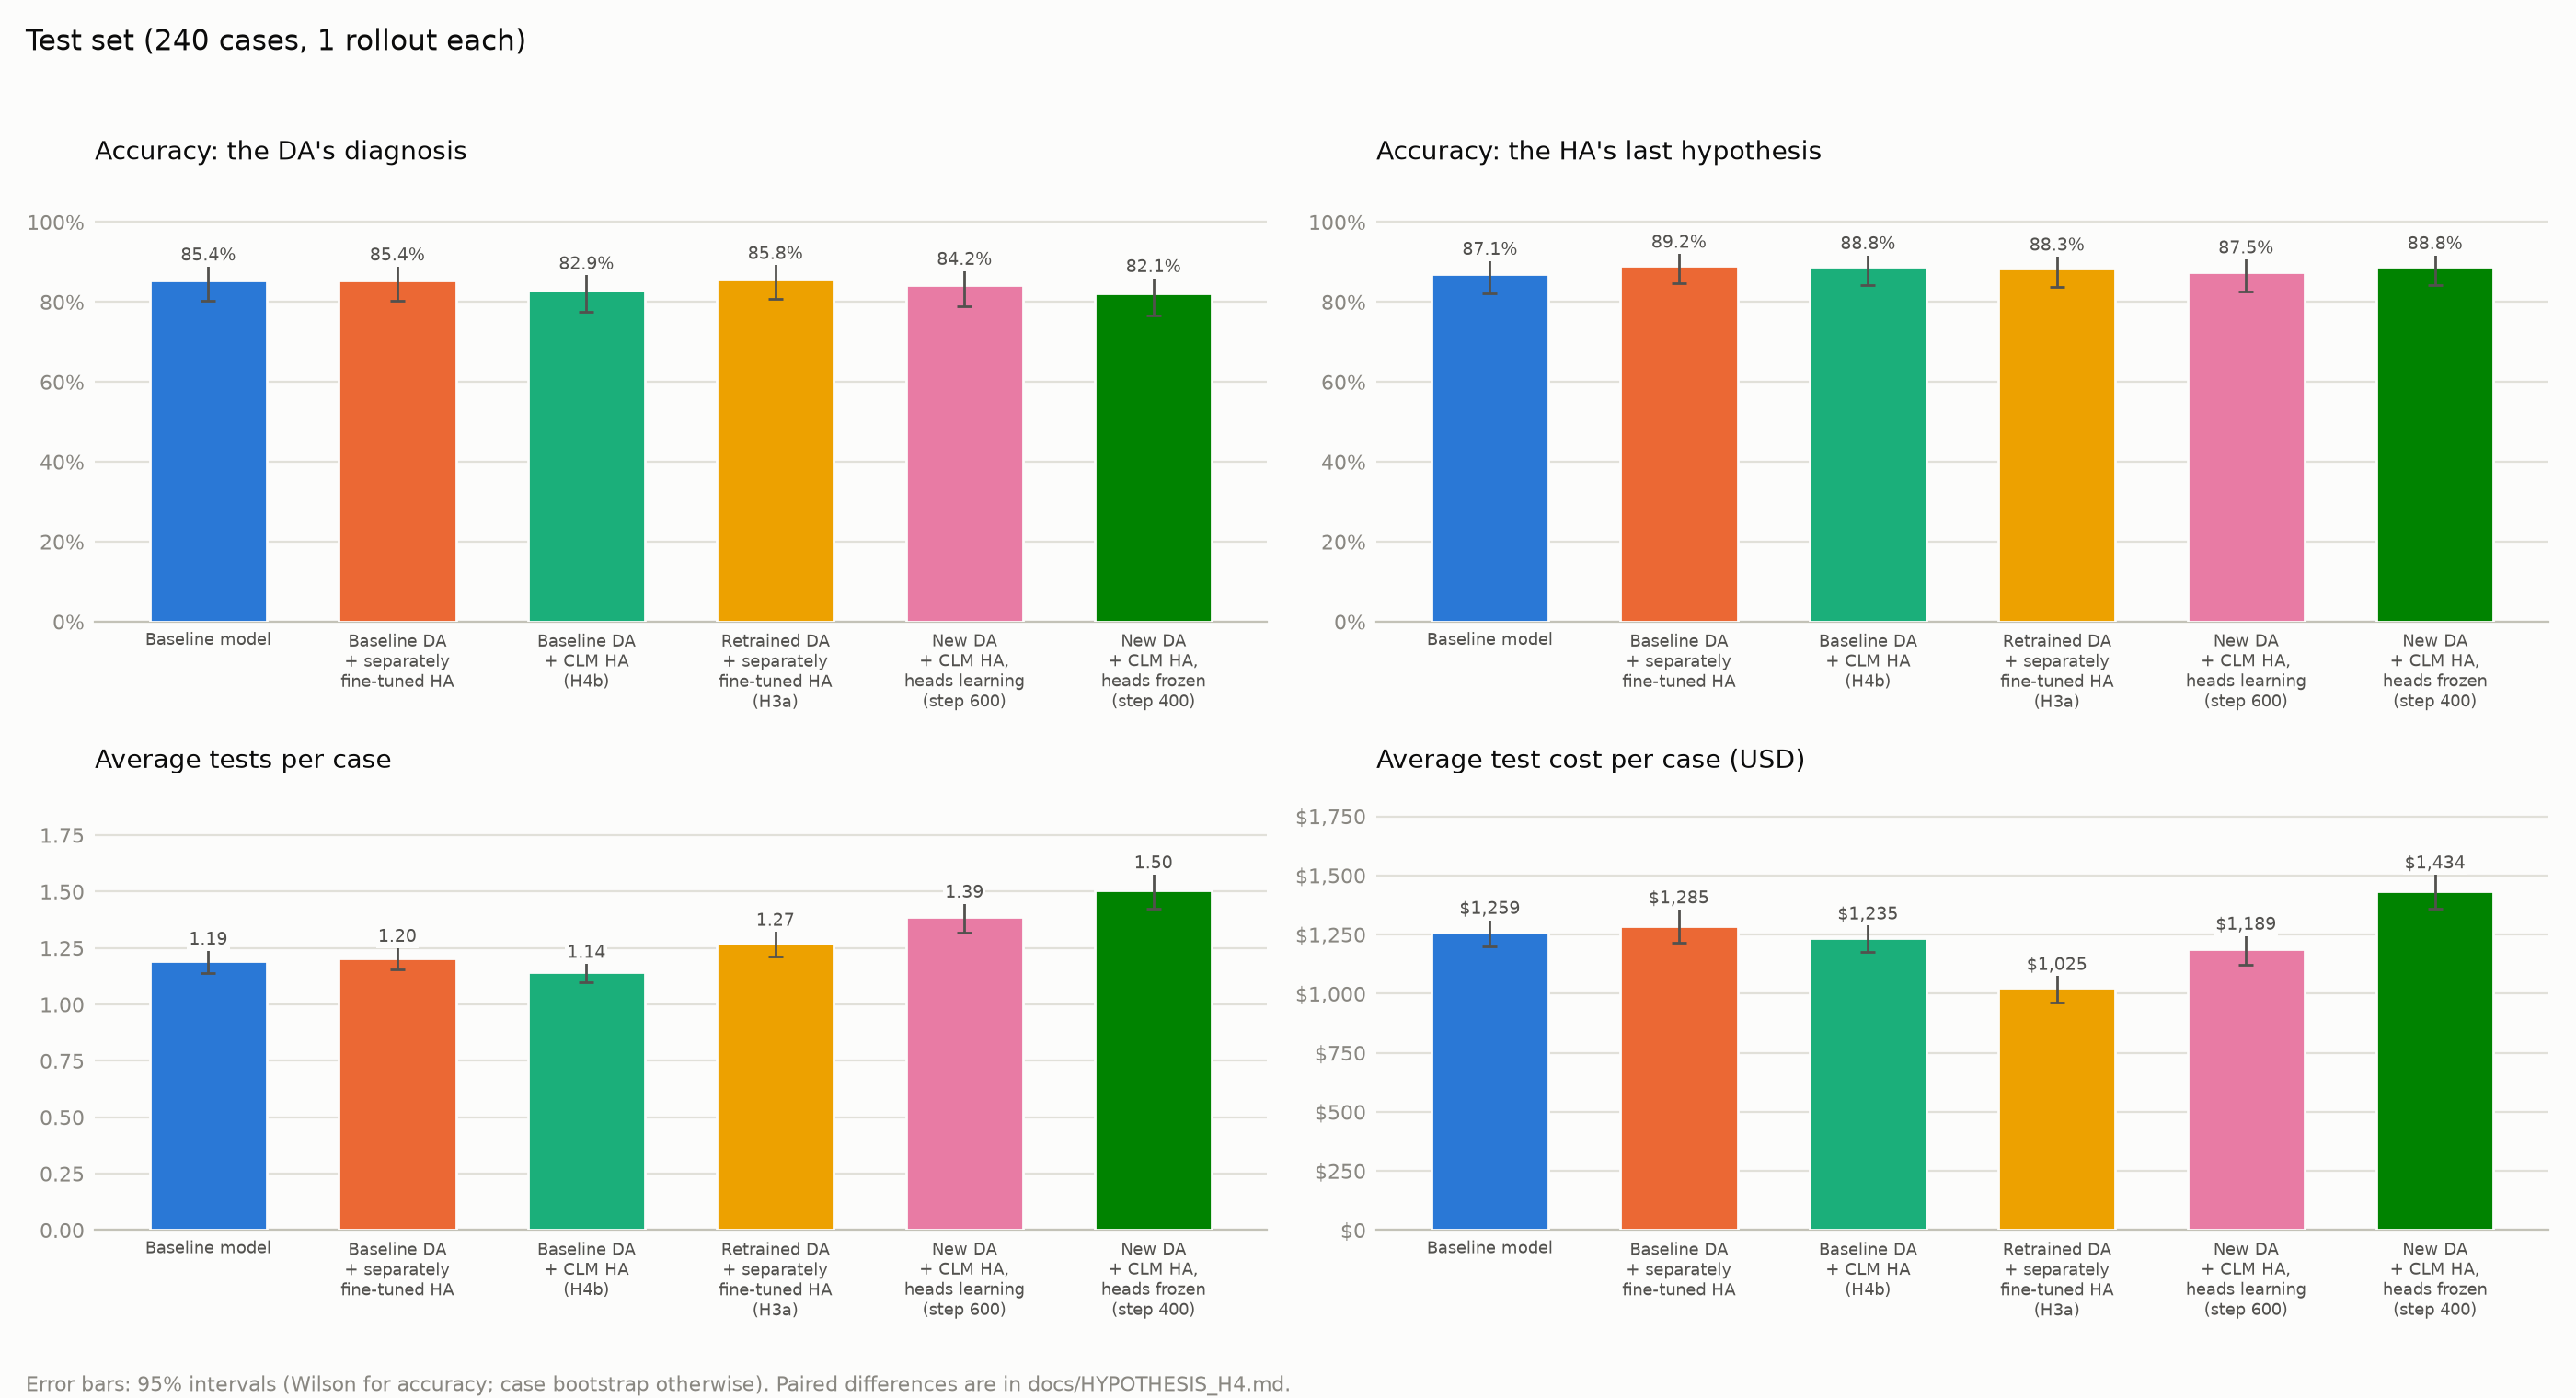
\includegraphics[width=\textwidth]{h4_test_overview.png}
  \caption{All test systems of H3 and H4 side by side, with 95\% intervals.
  Paired differences are given in the text.}
  \label{fig:h4test}
\end{figure}

\subsection*{What I Learned}

A contrastive HA built on a frozen language model is a practical diagnoser:
with only the small heads trained on top of our best HA, it matched that HA, and
on plain Llama it came within a few points of the baseline HA. Its real advantage, that it
can be updated cheaply while the DA trains, did not translate into a better
system. A likely reason is that there was little left for the HA to learn: its
online loss was already low, and in every system the HA's last hypothesis
(87--89\%) was as accurate as or more accurate than the DA's own diagnosis
(82--86\%, Figure~\ref{fig:h4test}). The remaining errors come from the DA,
through the tests it orders and the correct hypotheses it overrides. So far,
retraining the DA against a pre-trained, frozen HA (H3a) gives the best
trade-off: no detectable accuracy difference from any other system, at the
lowest cost.

\section{Challenges}
\label{sec:challenges}

\textbf{A resume bug, and a correction to Week 8.} After H4c I extended both
arms from 700 to 1,900 steps as an exploratory run. Right after resuming at
step 700, invalid action formats jumped from about 15\% to about 90\% in both
arms, and the DAs then relearned the format as if from scratch
(Figure~\ref{fig:bug}). The cause is a bug in the Hugging Face \texttt{Trainer}:
when a checkpoint holds a second adapter in a subfolder (here the frozen HA's),
it reloads only that subfolder adapter and never loads the DA's own adapter. A
resumed job therefore continued with an untrained DA while the step counter and
optimizer state were restored, so nothing reported an error. I fixed it with a
callback that reloads the DA's adapter after the Trainer's own loading, and a unit
test that checks the restored weights exactly.

This also changes a conclusion of Week 8. There I reported that the late-training
instability in H3 was not caused by the restart after the 24-hour limit. It was,
for the most part. H3a resumed at step 875 and was untrained at step 900, and H3b
resumed at step 700, dipped at step 800 and recovered by relearning. Only H3a's
drift towards ordering fewer tests at step 800 happened within one uninterrupted
job. The H3 and H4 results themselves are not affected: every chosen checkpoint
was saved before any resume. One qualification: H3b's steps 800 and 900 came
after its faulty resume, so its checkpoint was effectively chosen among steps
100--700. Given its 11-point deficit, a later checkpoint is unlikely to have
changed the H3b conclusion. The same applies to the team's observation that
validation accuracy falls after about a third of the training patients: the
large drop after step 700 was this bug, not overfitting.

\begin{figure}[htbp]
  \centering
  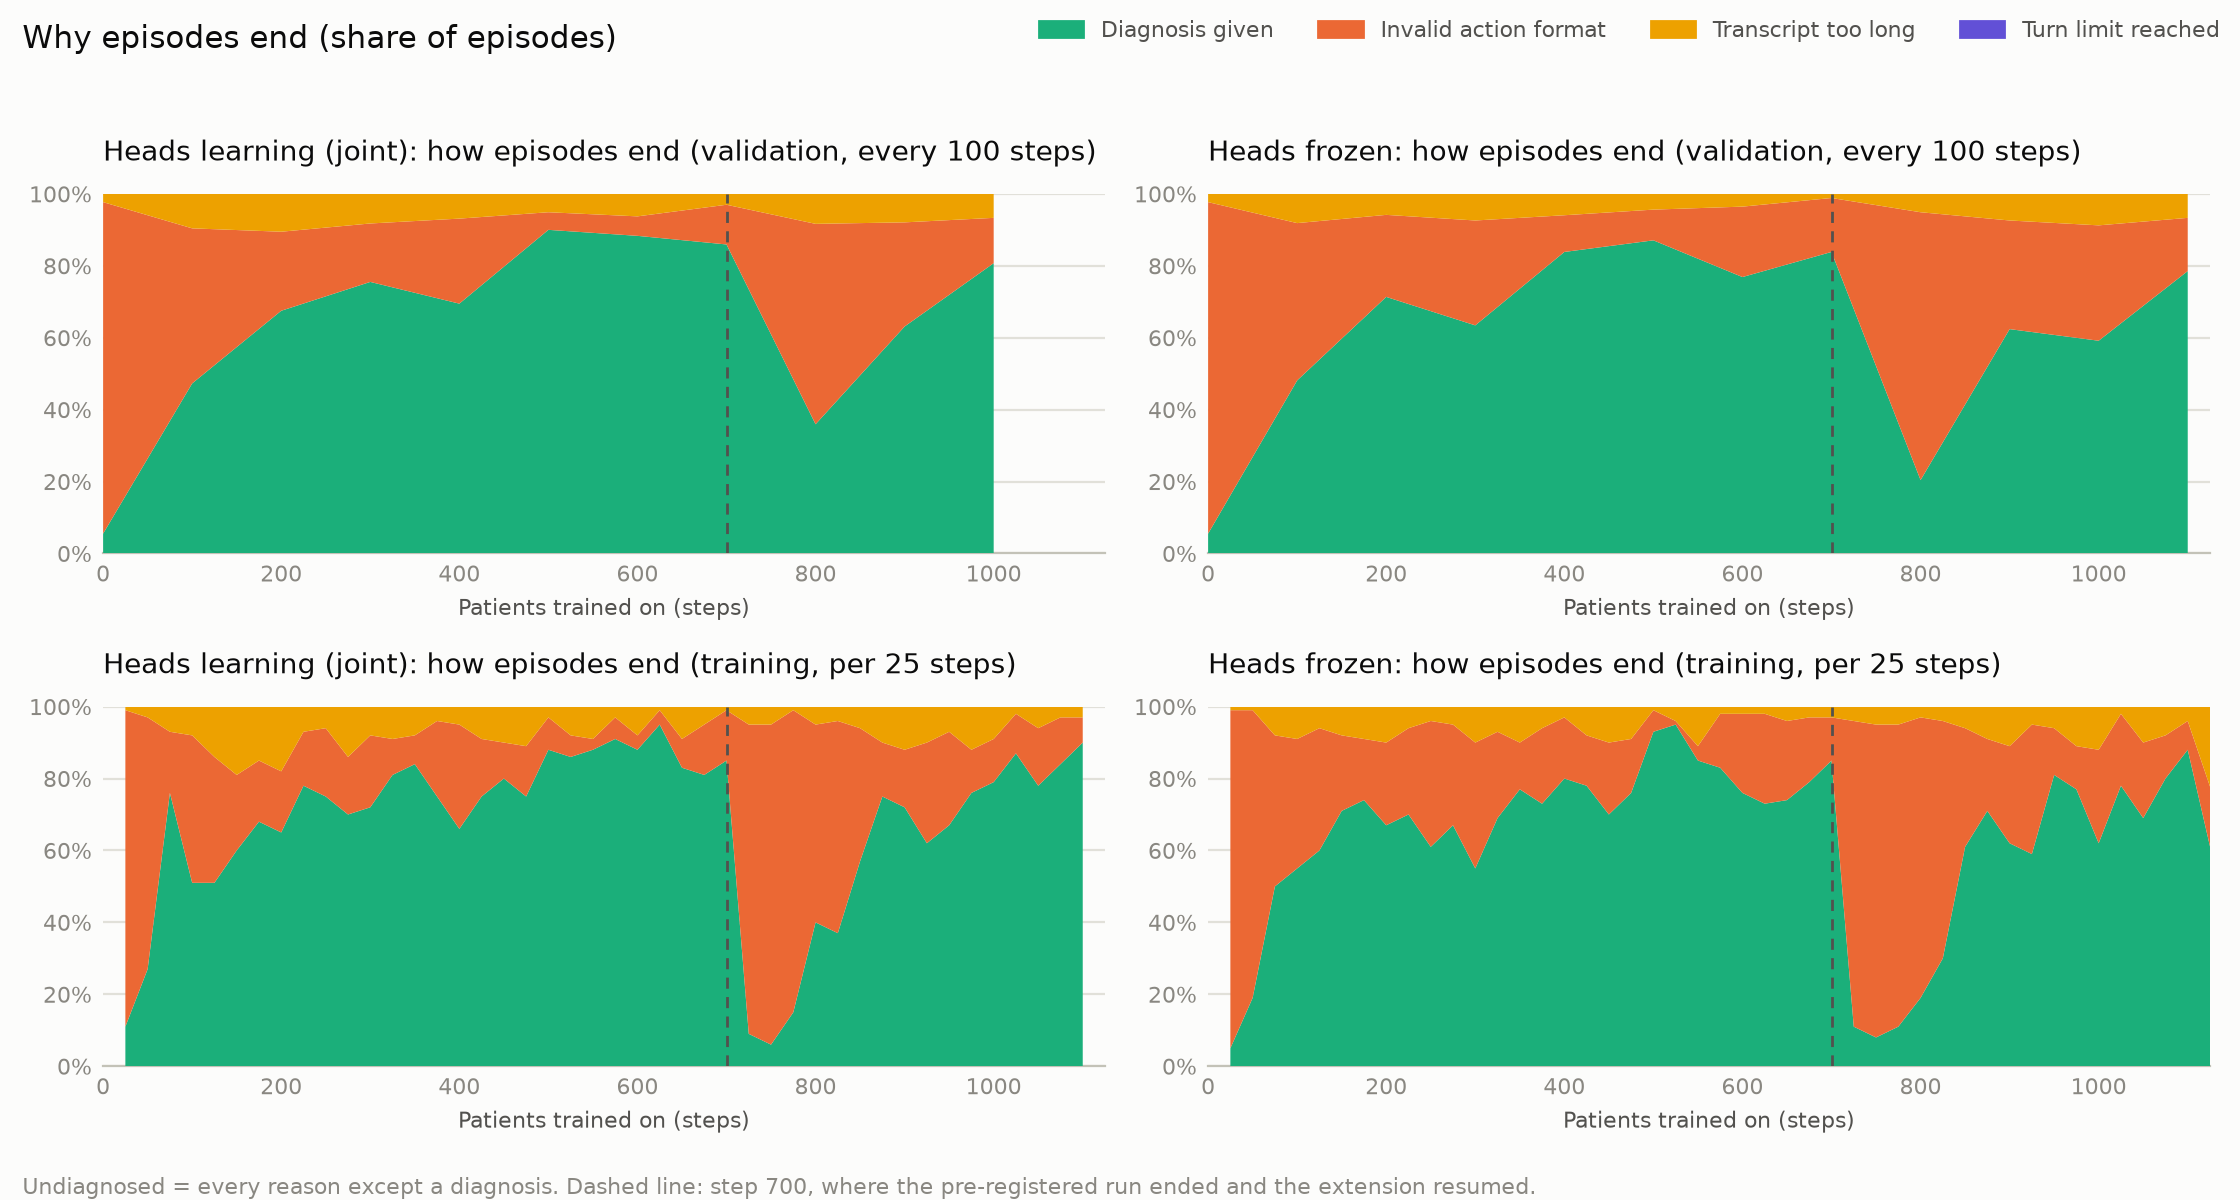
\includegraphics[width=\textwidth]{h4_end_reasons.png}
  \caption{How episodes ended in the first, invalid extension run. The dashed
  line marks step 700, where the job resumed with the untrained DA.}
  \label{fig:bug}
\end{figure}

\textbf{Restarting the extension.} The Trainer keeps only the five newest
checkpoints, so the step-700 checkpoint had already been deleted. I rebuilt it
from our own adapter snapshot at step 700, which has the exact DA and head
weights. Only the optimizer's running averages are lost, so they restart fresh.
The extension is running again and will be reported as exploratory; the 700-step
comparison remains the pre-registered result.

\textbf{Limits.} Each H4 arm is a single run, and the validation curves move by
5 to 13 points between checkpoints, which is as large as the effects being
tested. The 240-patient test set gives intervals of about $\pm$4--7 points for
paired differences.

\section{Next Steps: Towards the Final Submission}

This is the last weekly report; the team aims to submit the final work by
Sunday, November 29. Following this week's meeting, the CLM becomes the main
direction of the write-up. Before the submission I plan, in order of priority:

\begin{itemize}
  \item \textbf{DA--HA disagreement analysis} (no training): for every system,
        count how often the DA overrides a correct HA and how often it corrects
        a wrong one, and test the rules ``diagnose with the HA's final
        hypothesis'' and ``defer to the HA above a confidence threshold''. Any
        threshold will be chosen on validation episodes and evaluated once on
        test.
  \item \textbf{External validation:} run the fixed baseline, H3a and H4
        systems once on Edward's external test set (152 openly licensed
        published case reports, not MIMIC) to check how they generalise.
  \item \textbf{Confidence bounds for the HA} (suggested in this week's team
        meeting):
        train an ensemble of CLM heads, which takes minutes, to obtain lower
        and upper confidence bounds per disease, and test offline whether the
        bounds identify the HA's errors and support a ``diagnose or test more''
        rule.
  \item \textbf{Cheap ablations without training:} the DA evaluated with no HA
        messages, and a weaker DA (the untrained model) with the CLM HA.
  \item Finish the 1,900-step extension and report it as exploratory.
\end{itemize}

Ideas that need new DA training runs (bounds in the DA's input, a combined HA,
CLM-guided search, a contrastive DA, extra seeds) will be described as future
work unless the analyses above point clearly to one of them.

\section{AI Disclaimer}

I used Anthropic Claude to assist with designing the experiments, implementing
the code, inspecting training and evaluation logs, computing the statistics,
diagnosing the resume bug, and drafting this report.

\end{document}
